\subsection{Important Functions}
\begin{example}[Even]
	\hfill
	All of the examples have the point $(0, 0) \, (1,1) \, (-1,-1)$ except for the $f(x) = b$ which is just a constant value and the $f(x) = \sqrt{x}$ function which can't have a negative input ($x \ge 0$).
	\begin{enumerate}
		\item $$f(x) = b$$
			\begin{center}
			\textit{For this example $b = 1$}
			\end{center}
			\hfill
			\begin{center}
			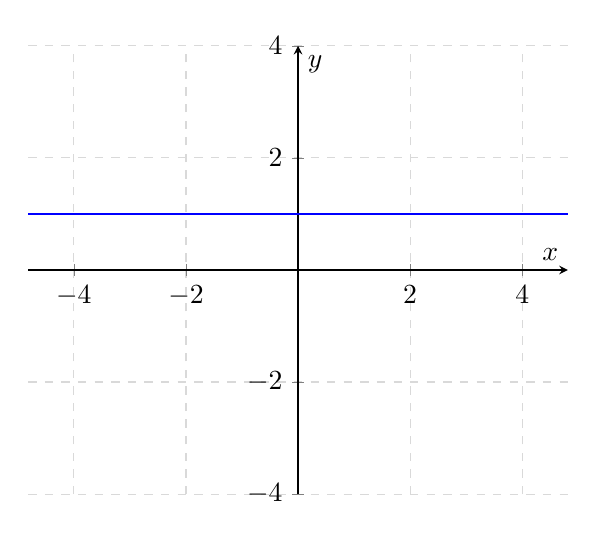
\begin{tikzpicture}
				\begin{axis}[
				    axis lines = center,
				    xlabel = $x$,
				    ylabel = $y$,
				    xmin = -4, xmax = 4,
				    ymin = -4, ymax = 4,
				    grid = both,
				    grid style = {dashed, gray!30},
				    axis equal
				]
				    \addplot [domain=-5:5, samples=100, thick, blue] {1};
				\end{axis}
			\end{tikzpicture}
			\end{center}
		\item $$f(x) = x^2$$
			\hfill
			\begin{center}
			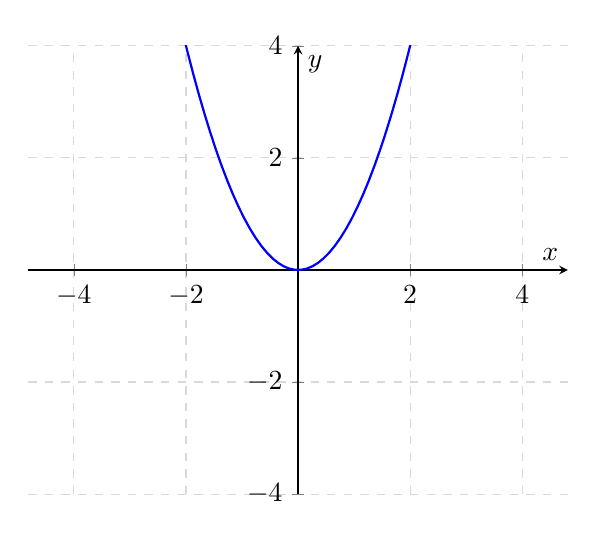
\begin{tikzpicture}
				\begin{axis}[
				    axis lines = center,
				    xlabel = $x$,
				    ylabel = $y$,
				    xmin = -4, xmax = 4,
				    ymin = -4, ymax = 4,
				    grid = both,
				    grid style = {dashed, gray!30},
				    axis equal
				]
				    \addplot [domain=-5:5, samples=100, thick, blue] {x^2};
				\end{axis}
			\end{tikzpicture}
			\end{center}
		\item $$f(x) = |x|$$
			\hfill
			\begin{center}
			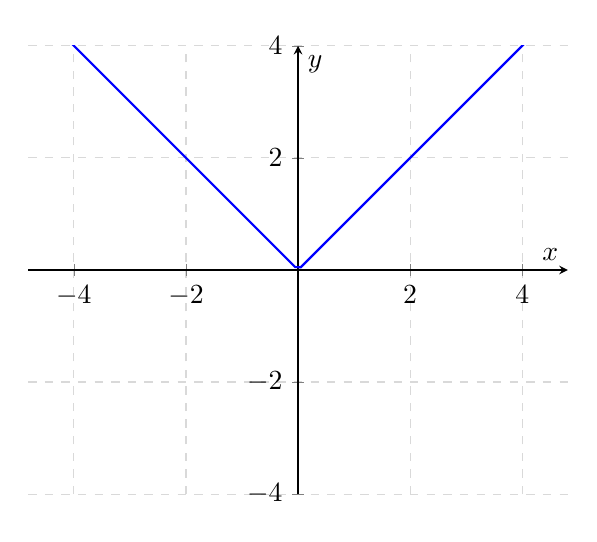
\begin{tikzpicture}
				\begin{axis}[
				    axis lines = center,
				    xlabel = $x$,
				    ylabel = $y$,
				    xmin = -4, xmax = 4,
				    ymin = -4, ymax = 4,
				    grid = both,
				    grid style = {dashed, gray!30},
				    axis equal
				]
				    \addplot [domain=-5:5, samples=100, thick, blue] {abs(x)};
				\end{axis}
			\end{tikzpicture}
			\end{center}
		\item $$f(x) = \sqrt{x}$$
			\hfill
			\begin{center}
			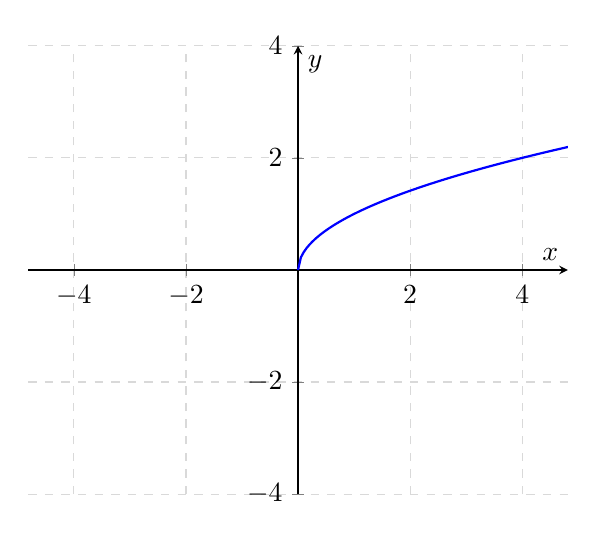
\begin{tikzpicture}
				\begin{axis}[
				    axis lines = center,
				    xlabel = $x$,
				    ylabel = $y$,
				    xmin = -4, xmax = 4,
				    ymin = -4, ymax = 4,
				    grid = both,
				    grid style = {dashed, gray!30},
				    axis equal
				]
				    \addplot [domain=0:5, samples=100, thick, blue] {sqrt(x)};
				\end{axis}
			\end{tikzpicture}
			\end{center}
	\end{enumerate}
\end{example}

\begin{example}[Odd]
	\hfill
	All of the examples have the point $(0, 0) \, (1,1) \, (-1,-1)$ except for the $f(x) = \frac{1}{x}$ function which doesn't have the $(0, 0)$ point.
	\item $$f(x) = x$$
			\hfill
			\begin{center}
			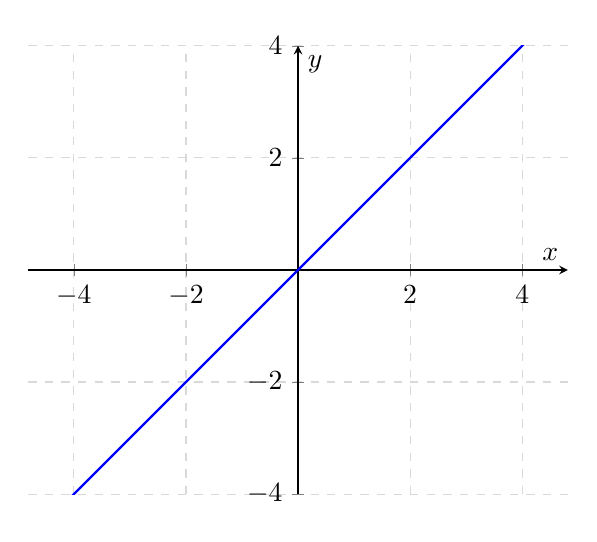
\begin{tikzpicture}
				\begin{axis}[
				    axis lines = center,
				    xlabel = $x$,
				    ylabel = $y$,
				    xmin = -4, xmax = 4,
				    ymin = -4, ymax = 4,
				    grid = both,
				    grid style = {dashed, gray!30},
				    axis equal
				]
				    \addplot [domain=-5:5, samples=100, thick, blue] {x};
				\end{axis}
			\end{tikzpicture}
			\end{center}
	\item $$f(x) = x^3$$
			\hfill
			\begin{center}
			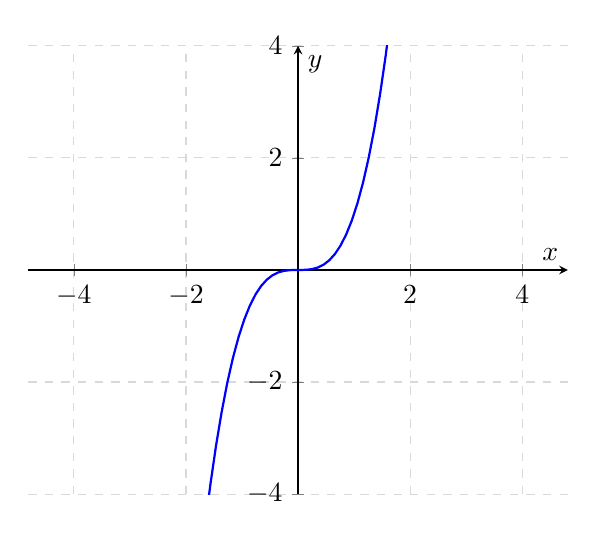
\begin{tikzpicture}
				\begin{axis}[
				    axis lines = center,
				    xlabel = $x$,
				    ylabel = $y$,
				    xmin = -4, xmax = 4,
				    ymin = -4, ymax = 4,
				    grid = both,
				    grid style = {dashed, gray!30},
				    axis equal
				]
				    \addplot [domain=-5:5, samples=100, thick, blue] {x^3};
				\end{axis}
			\end{tikzpicture}
			\end{center}
	\item $$f(x) = \sqrt[3]{x}$$
			\hfill
			\begin{center}
			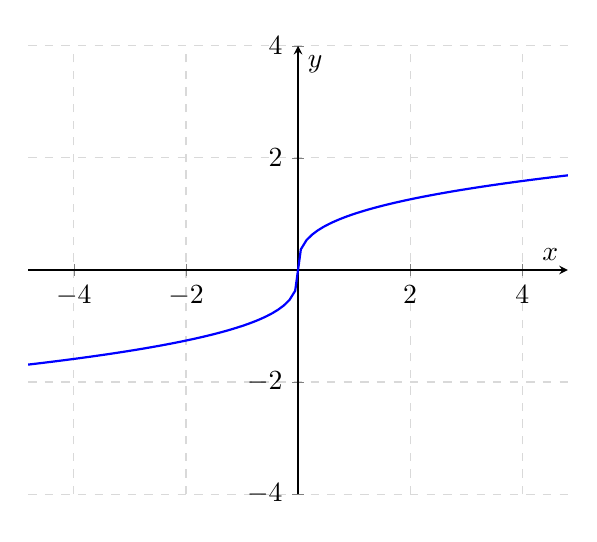
\begin{tikzpicture}
				\begin{axis}[
				    axis lines = center,
				    xlabel = $x$,
				    ylabel = $y$,
				    xmin = -4, xmax = 4,
				    ymin = -4, ymax = 4,
				    grid = both,
				    grid style = {dashed, gray!30},
				    axis equal
				]
					% Equivalent to cubic root
				    \addplot [domain=-5:5, samples=100, thick, blue] {sign(x)*abs(x)^(1/3)};
				\end{axis}
			\end{tikzpicture}
			\end{center}
	\item $$f(x) = \frac{1}{x}$$
			\hfill
			\begin{center}
			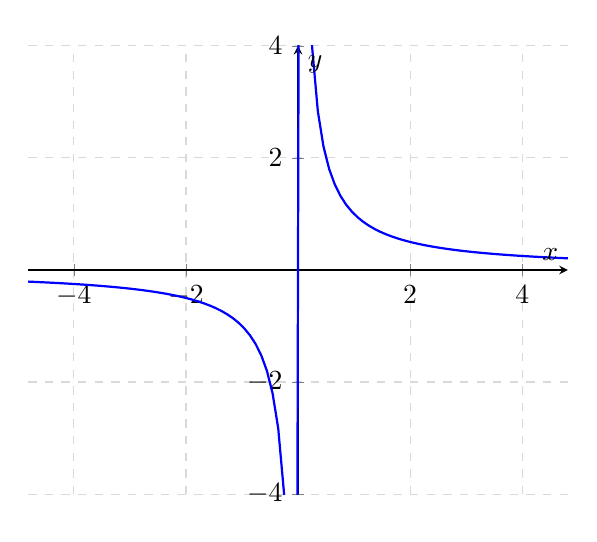
\begin{tikzpicture}
				\begin{axis}[
				    axis lines = center,
				    xlabel = $x$,
				    ylabel = $y$,
				    xmin = -4, xmax = 4,
				    ymin = -4, ymax = 4,
				    grid = both,
				    grid style = {dashed, gray!30},
				    axis equal
				]
				    \addplot [domain=-5:5, samples=100, thick, blue] {1/x};
				\end{axis}
			\end{tikzpicture}
			\end{center}
\end{example}
